\documentclass{../template/tp}
\usepackage[utf8]{inputenc}
\usepackage{ucs}
\usepackage[frenchb]{babel}
\usepackage[T1]{fontenc}

\usepackage{graphicx}
\usepackage{amssymb}
\usepackage{amsmath}
\usepackage{wasysym} %smiley
\usepackage{hyperref}% hyperliens
\usepackage{tikz}
\usetikzlibrary{babel,positioning,calc}
\usepackage[]{circuitikz}
\usepackage{textcomp}
% \usepackage{minted}
\usepackage[long]{datetime}
\usepackage{gensymb} % \ohm, celsius
\usepackage{framed}
\usepackage{pdfpages}
\usepackage{mathastext} % math as standfard text : units are respecting typography conventions.
\usepackage{xspace} % typographie IN
\usepackage[all]{hypcap} %lien pointe en haut des figures
\langexam{frenchb}
\usepackage{fancyhdr}

\newboolean{koriG}
\ifx\koriG\undefined
\correction{false}
\else
\correction{true}
\fi

\author{The Fantastic Four}


\newcommand{\itgv}[1]{\ifthenelse{\boolean{corrige}}{{\color{blue}#1}}{}} %si corrigé vrai...
\newcommand{\ifgv}[1]{\ifthenelse{\boolean{corrige}}{}{#1}} %si corrigé vrai...
%% fancy header & foot
\pagestyle{fancy}
\lhead{[ELEC-H-301] Électronique appliquée\\ TP \no 5 : transistors MOS}
\rhead{v1.0.0\\ page \thepage}
\chead{\ifthenelse{\boolean{corrige}}{Corrigé}{}}
\cfoot{}
%%

\pdfinfo{
/Author (Yannick Allard, ULB -- BEAMS)
/Title (TP 5 ELEC-H-301, transistors MOS)
/ModDate (D:\pdfdate)
}

\hypersetup{
pdftitle={TP 5 [ELEC-H-301] Électronique appliquée : transistors MOS},
pdfauthor={Yannick Allard, ©2016 ULB - BEAMS  },
pdfsubject={Transistor MOS}
}

%\date{\vspace{-1cm}\mydate\today}
%\title{\vspace{-2cm} Labo \no 6\\ Électronique appliquée [ELEC-H-301]\\Réalisation d'un ampli à transistor\ifthenelse{\boolean{corrige}}{~\\Corrigé}{}}

%\author{\vspace{-1cm}}%\textsc{Yannick Allard}}

\setlength{\parskip}{0.4cm plus1mm minus1mm} %espacement entre §
\setlength{\parindent}{0pt}
\setlength{\headheight}{30pt}


\begin{document}

\tptitle{ELEC-H-301~: Électronique appliquée}{Séance 5~: les transistors MOS}
\ifthenelse{\boolean{corrige}}{\vspace{-2cm}}{}
\section{Introduction}
\subsection{But}
Le but de ce TP est de vous rafraîchir la mémoire sur les transistors MOS et de vous préparer efficacement au labo \no 4. Ce TP fait office de prédéterminations pour le labo.
\subsection{Prérequis}
Avoir lu et compris le chapitre 18 (ed 5) du support de cours portant sur les transistors MOS.

Avoir trouvé la documentation des transistors utilisés dans cette séance d'exercices.

\subsection{Objectifs}
À la fin de ce TP, vous devrez être capable :
\begin{itemize}
\item d'utiliser les notations des grandeurs liées au transistor MOS
\item comprendre comment utiliser une source de courant commandée en tension pour réaliser un amplificateur tension--tension
\item de comprendre la polarisation du transistor MOS et ses conséquences sur le point de fonctionnement %(= caractéristiques à petit signal)
\item de réaliser un schéma à petit signal d'un montage à transistor
\item d'extraire les paramètres intéressants de la documentation d'un transistor en vue de dimensionner un étage
\item d'aborder sereinement des exercices de dimensionnement et le laboratoire portant sur le transistor MOS.
\end{itemize}
\subsection{Lexique}
%\section{Get ready, Set! Go!!!!}
\begin{center}
\begin{footnotesize}
\begin{tabular}{rl|rl}
\textit{Gate} & Grille 		& \textit{Operating point	} & point de fonctionnement \\
\textit{Source} & Source 	& \textit{Coupling capacitor} & capacité de couplage\\ 
\textit{Drain} & Drain 		& \textit{Common source amplifier} & amplificateur à source commune\\
\textit{Load line} & droite de charge & \textit{Quiescent drain current} & courant de drain statique \\ 
& & \textit{Power dissipation} & puissance dissipée \\
\end{tabular} 
\end{footnotesize}
\end{center}
\newpage
\section{Notations}
L’objectif de cette question est de vous familiariser avec les notations des différentes grandeurs électriques liées à l'utilisation d'un transistor MOS.

Soit le schéma électrique du transistor MOS et son équivalent à petit signal~:

\ifthenelse{\boolean{corrige}}{ %if, then
\begin{center}
%\shorthandoff{:!}
\color{blue}
		\begin{circuitikz} \draw
		(2.25, 1) node[nfet] (mos) {}
%		(0,0) -- (2,2)
%		(0,0) node[nfet]{} -- (2,2)
		%(mos.B) node[anchor=west] {B}
		%(mos.G) node[anchor=east] {}		
		(mos.D) -- (2.25, 2) to  [short, -o, i<=$I_D$](3.25, 2)  node[anchor=west] {D} %D		
		(mos.S) -- (2.25, 0) to [short, -o](3.25, 0)  node[anchor=west] {S} %S		
		(mos.B) -- (mos.S)
		(2.25,0) to [short, -o](0,0)  node[anchor=east] {S} %S		
		(0,2)  node[anchor=east]{G}[short, o-] to  (1,2) %G
		(1,2) -- (1,1) -- (mos.G)
		(0,0) [open,v^>=$V_{GS}$] to (0,2)
		(3.25,0) [open,v>=$V_{DS}$] to (3.25,2)
		%(gin) -- (mos.G)
		;\end{circuitikz}\hspace*{1cm}
		\begin{circuitikz}\draw
		(0,0) node[anchor=east] {g} %g
		to [short, o-] (1,0) 
		to [open, v<=$v_{gs}$] (1,-2)
		to [short, -o] (4,-2)
		to [short, -o] (0,-2) node[anchor=east] {s} %s
		%to [short] (3,-2)
		(3,0) to [cI, i_=\rotatebox{90}{$g_m\cdot v_{gs}$}] (3,-2)
		(3,-2) to [short, -o] (4,-2) node[anchor=west] {s} %s
		(3,0) to [short, -o] (4,0)
		to node[anchor=west] {d} (4,0) %d
		(4.0,-2) [open,v>=$v_{ds}$] to (4.0,0)
	;\end{circuitikz}
%\shorthandon{:!}		
	\end{center}
} %/then
{ %else
\begin{center}
%\shorthandoff{:!}
		\begin{circuitikz} \draw
		(2.25, 1) node[nfet] (mos) {}
%		(0,0) -- (2,2)
%		(0,0) node[nfet]{} -- (2,2)
		%(mos.B) node[anchor=west] {B}
		%(mos.G) node[anchor=east] {}		
		(mos.D) -- (2.25, 2) to  [short, -o](3.25, 2)  node[anchor=west] {} %D		
		(mos.S) -- (2.25, 0) to [short, -o](3.25, 0)  node[anchor=west] { } %S		
		(mos.B) -- (mos.S)
		(2.25,0) to [short, -o](0,0)  node[anchor=east] {} %S		
		(0,2)  node[anchor=east]{}[short, o-] to  (1,2) %G
		(1,2) -- (1,1) -- (mos.G)
		%(gin) -- (mos.G)
		;\end{circuitikz}\hspace*{1cm}
		\begin{circuitikz}\draw
		(0,0) node[anchor=east] {} %g
		to [short, o-] (1,0) 
		to [open, v<={~}] (1,-2)
		to [short, -o] (4,-2)
		to [short, -o] (0,-2) node[anchor=east] {} %s
		%to [short] (3,-2)
		(3,0) to [cI, i={~}] (3,-2)
		(3,-2) to [short, -o] (4,-2) node[anchor=west] {} %s
		(3,0) to [short, -o] (4,0)
		to node[anchor=west] {} (4,0) %d
	;\end{circuitikz}
%\shorthandon{:!}		
	\end{center}
} %/else

	%\vspace*{-0.5cm}
\Question{~\\%~\\ %sinon, ça fait dlm
\begin{itemize}
\item Identifier les ports des deux schémas.
\item Remplir le tableau suivant et indiquer les grandeurs sur le schéma.\vspace{-1.5Em}
\end{itemize}



\begin{center}
\begin{tabular}{|c|l|c|c|}
\hline 
{grandeur} &{\hspace*{1cm}nom\hspace*{1cm}}--{\hspace*{2cm}signification\hspace*{2cm}} & {statique} & {dynamique}\\ 
\hline 
$V_{GS}$ &  \itgv{tension de polarisation grille--source (V)}  & \itgv{x} &  \\ [1.5em]
\hline
$v_{gs}$ &  \itgv{tension G--S à petit signal (V)}  &  & \itgv{x} \\ [1.5em]
\hline
$V_{DS}$ &  \itgv{tension de polarisation D--S (V)}  & \itgv{x} &  \\ [1.5em]
\hline
$v_{ds}$ &  \itgv{tension D--S à p.s. (V)}  &  & \itgv{x} \\ [1.5em]
\hline
$I_{D}$ &  \itgv{courant de drain statique (A)}  & \itgv{x} &  \\ [1.5em]
\hline 
$g_{m}$ &  \itgv{transconductance du transistor (A/V=S)}  &  & \itgv{x} \\ [1.5em]
\hline 
$g_{m}\cdot v_{gs}$ &  \itgv{courant de drain à petit signal (A)}  &  & \itgv{x} \\ [1.5em]
\hline 
\end{tabular} 
\end{center}
}%
{ Voir table.
}
\newpage
\section{Amplifier avec une source de courant commandée idéale }
Afin de réaliser un amplificateur \textbf{tension--tension}, on se propose d'utiliser un transistor MOS. 
%
Or le transistor MOS se comporte comme une source de \textbf{courant} -- non idéale -- commandée en tension et ne peut donc pas être utilisé immédiatement pour réaliser une source de tension commandée en tension. En pratique, lorsque le point de fonctionnement est correctement choisi, la source non-idéale a un comportement presque idéal.
%
%L'intérêt du transistor MOS est de se comporter comme une source de \textbf{courant} commandée en tension, malheureusement imparfaite. %Dans un premier temps, considérons une source idéale.
%
%Voyons d'abord comment construire un amplificateur tension--tension en utilisant une source de courant commandée en tension \textit{idéale}.
%
%La première étape sera d'amplifier de tension à tension en utilisant une source de courant \textit{idéale} commandée en tension.
%
La source \textit{idéale} utilisée est représentée figure \ref{fig:source}\footnote{NB : le symbole européen de la source de courant commandée est utilisé ici}.
%
\begin{figure}[h!]
	\begin{center}
		\begin{circuitikz}\draw
			(0,0) node[anchor=east] {g} 
			to [short, o-] (1,0) 
			to [open, v<=$v_{gs}$] (1,-2)
			to [short, -o] (0,-2)
			to  (0,-2) node[anchor=east] {s}
			%to [short] (3,-2)
			(3,0) to [cI=$ g \cdot v_{gs}$] (3,-2)
			(3,-2) to [short, -o] (4,-2) node[anchor=west] {s}
			(3,0) to [short, -o] (4,0)
			to node[anchor=west] {d} (4,0)
			(1,-2) -- (3,-2)
		;\end{circuitikz}
	\end{center}
\caption{Source de courant commandée en tension}
\label{fig:source}
\end{figure}


%\subsection{Caractéristique de transfert de cette source commandée idéale}
%équations + courbes ??

Cette source \textit{idéale} absorbe un courant proportionnel à la tension d'entrée selon la~loi : $$i_d = g \cdot v_{gs}$$

où $g$ est la transconductance de la source. 


\Question{
\begin{itemize}
\item À quelle condition cette source est-elle linéaire ?
\item Tracer sa caractéristique de transfert.
\item Que faut-il ajouter pour obtenir un amplificateur tension--tension.
\end{itemize}
	
	\label{Q:1}
	
	}
	{
	\begin{itemize}
		\item $g$ doit être constante par rapport à $v_{gs}$.
		\item $i_d=f(v_{gs})$\\
			\begin{tikzpicture}[domain=-5:5]
		    \draw[very thin,color=gray,xstep=1, ystep=0.1] (-4,-1.05) grid (4,1);
		    \draw[->, thick] (-4.2,0) -- (4.2,0) node[right] {$v_{gs}$};
		    \draw[->, thick] (0,-1.2) -- (0,1.2) node[above] {$i_d$};
		    \draw[color=red,thick] plot[id=x] function{0.2*x} 
		        node[right] {$i_d(v_{gs})$};
		%    \draw[color=blue] plot[id=sin] function{sin(x)} 
		 %       node[right] {$f(x) = \sin x$};
		  %  \draw[color=orange] plot[id=exp] function{0.05*exp(x)} 
		   %     node[right] {$f(x) = \frac{1}{20} \mathrm e^x$};
		\end{tikzpicture}
		\item il faut ajouter une résistance pour \og convertir \fg le courant en tension. Il faut la mettre en parallèle avec la source de courant (source de Norton).
		\end{itemize}	
	
	}
	
	\newpage
\section{Polarisation et point de fonctionnement}

\Question {
Rappel TP3 : résoudre ce circuit à AOP avec polarisation (En considérant que les condensateurs se comportent comme des court-circuits à la fréquence de la source $v_{in}$) :
\begin{center}
 

 \begin{circuitikz} [scale=1.2]\draw
 (0,0) node[op amp] (opamp) {}
% (opamp.+) node[left] {$v_+$}
% (opamp.-) node[left] {$v_-$}
% (opamp.out) node[right] {$v_o$}
 (opamp.down) ++ (0,-0.5) node[below] {-12V} -- (opamp.down)
 (opamp.up) ++ (0,.5) node[above] {12V} -- (opamp.up)
 (opamp.-) -| (-1.5,2) to [R, l=$R2$] (1.5,2) |-  (opamp.out)
 (opamp.+) -| (-1.5,-0.4) to [european voltage source, l_=$V_{C}$,-*] (-1.5,-2) node[ground] {} 
 (-4,-2) node[ground] {}  to [sV,*-*] (-4,0.4) |- ++(0.5,0) to [C,l=$C1$] ++(0.25,0) to [R,l=$R1$] (opamp.-)
 (-4,-2) node[anchor=west] {\itgv{$0V$}}
 (-1.5,-2) node[anchor=west] {\itgv{$0V$}}
 (-2.9,0.4) node[circ]{}
 (-2.9,0.4) node[anchor=south]{\rotatebox{90}{\itgv{$6.3V+v_{in}$}}}
 (-1.5,0.4) node[circ]{}
 (-1.5,0.4) node[anchor=south west]{\rotatebox{42}{\itgv{$6.3V$}}}
 (-1.5,-0.4) node[circ]{}
 (-1.5,-0.4) node[anchor=east]{\itgv{$6.3V$}}
 (1.5,0) node[circ]{}
 (1.5,0) node[anchor=south west]{\itgv{$6.3V-10v_{in}$}}
 (opamp.out) to (2.5,0)
 (2.5,-2) node[ground] {} to [open, v>=$V_{out}$] (2.5,0)
 (-4.5,-2) to [open, v^>=$v_{in}$] (-4.5,0.5)
 (-4,0.4) node[anchor=east] {\itgv{$v_{in}$}}
% (-1.5,-2)

 ;\end{circuitikz}

\end{center}
$R1=1k\Omega$, $R2=10k\Omega$, $C1=1\mu F$, $v_{in}=0.42 sin(\omega t) V$, $V_C=6.3V$

\begin{itemize}
\item Calculer les tensions en tout point du circuit.
\end{itemize}


}
{Dans le cas où $\frac{1}{j\cdot C1\omega}\ll R1$, voir schéma.

}

\Question{
\label{Q:ex4}
Soit le circuit suivant :
\begin{center}
			%\includegraphics[width=8cm]{}
			\begin{circuitikz}[scale=1]\draw
			(0,1) to [short,o-] (9,1)
			(4,6) to [short] (9,6)
			(0,3) node[anchor=east] {In} to [short,o-] (1,3)
			(0,3) node[anchor=south]{\itgv{$0V$}} to [open, v_<=$V_{in}$]  (0,1) 
			(1,3) to [C=$C_{in}$ ](1.5,3) 
			(1.5,3) to [short,-*] (2,3) node[anchor=south west]{\itgv{$3.1V$}}
	%
			(2,6) node[anchor=south ] (alim) {$+V_{DC}$}
			(1.6,6) -- (2.4,6) %bar under the label
			%(alim.text) node {}
	%		
			(2,3) to [R, l_=$R_{B1}$, i<=\itgv{$31\mu A$}](2,6)
			(2,3) to [R=$R_{B2}$](2,1)
	%		
			(4,3) node[nfet] (mos) {}
			%(mos.B) node[anchor=west] {B}
			(mos.G) to [short] (2,3)
	%		
			(mos.D) to (4,4) to [R, l_=$R_D$, i<=\itgv{$67mA$}] (4, 6)		
			%(4,5.5) to [R] (mos.D)
	%		
			(mos.D) to [short,-*](4,3.5)  to [short] (4.25,3.5)
	%		
			(mos.S) to [short] (4,1)% to [short, -o](2,0)  node[anchor=west] {S}
			(mos.S) -- (mos.B) %source to bulk connection		
	
			(4.25,3.5) node[anchor=south]{\rotatebox{80}{\itgv{$5.3V$}}} to [C, l^=$C{out}$] (6,3.5) to  [short](6,3.5)node[anchor=south]{\rotatebox{80}{\itgv{$0V$}}} to [short,-o](6.5,3.5)node [anchor=south] {Out}	
			(6,3.5) to [generic, l_=$R_{ch}$] (6,1)
			(6.5,3.5) to [open,v^<=$V_{out}$] (6.5,1)
	%		
			(9,6) to [battery, l_=$E$](9,1)
			
			%\ithenelse{\boolen{corrige}}{
			(4,1) node[circ]{}
			%}{}
			(4,1) node[anchor=south west]{\itgv{$0V$}}
			(4,6) node[anchor=south west]{\itgv{$12V$}}
			(2,5) node[anchor=south west]{\itgv{$6.2V$}}
	%		%(1,0) to [short, -o](-1,0)  node[anchor=east] {S}
	%		
	%%			(0,0) node[anchor=east] {In} 
	%%			to [short, o-] (1,0) 
	%%			to [open, v=$V_{GS}$] (1,-2)
	%%			to [short, -o] (0,-2)
	%%			to  (0,-2) node[anchor=east] {S}
	%%			to [short] (3,-2)
	%%			(3,0) to [cI=$ g_m \cdot V_{GS}$] (3,-2)
	%%			(3,-2) to [short, -o] (4,-2) node[anchor=west] {S}
	%%			(3,0) to [short, -o] (4,0)
	%%			to node[anchor=west] {D} (4,0)
	%	%		
			;\end{circuitikz}
	\end{center}
	
	Valeurs des composants/sources : 	$V_{DC}=6.2V$, $R_{B1}=R_{B2}=100k\Omega$, $R_D=100\Omega$, $C_{in}=100nF$, $C_{out}=2.2\mu F$, $E=12V$, $R_{ch}=3.3k\Omega$, $V_{in}$ sinusoïdale
	
	\begin{itemize}
	\item Calculer les tensions et courants \textbf{continus} en tout point du circuit. 
	\item Placer le point de fonctionnement sur les courbes caractéristiques du BS170 en annexe, en déduire $I_D$ et $g_m$.
	\item Tracer également la droite de charge et indiquer les limites de linéarité. % statique.
	\end{itemize}
	
	
	
	}
	{%
	Voir schéma ci dessus et courbes en annexe.
	
	Pour $V_{GS}=3.1V, I_D=67mA$, $g_m=197mS$.
	}

\ifgv{\newpage}

%TODO : ajouter droite de charge
%TODO : qqch fait dlm avec l'espace avant itemize FIXED

\section{Schéma à petit signal}

\Question
{
%question
Sachant que $V_{DC}$ a été judicieusement choisie pour obtenir $g_m=0.197S$ :
 
 \begin{itemize}
 \item Déterminer le schéma à petit signal du montage présenté à la question précédente.
 \item Calculer le gain du montage dans la bande passante. Les condensateurs peuvent être assimilés à des court-circuits dans la bande passante du montage.
 \item Calculer les impédances d'entrée et de sortie du montage.
 \item Donner l'expression des impédances d'entrée et de sortie pour toute fréquence (\textit{i.e.} l'approximation du premier point n'est plus valable).
 \item Calculer la fréquence de coupure à l'entrée et à la sortie du montage.
 \item Bonus : Établir la fonction de transfert complète du montage. Quel est le comportement de ce montage ?
 %\item Bonus : en considérant l'entrée du transistor MOS comme une capacité de $1pF$, calculer la fréquence de coupure haute du montage.ainsi que le gain pour toute fréquence
 \end{itemize}

}
{%answer

\begin{itemize}
\item Schéma à petit signal :
\begin{center}
			%\includegraphics[width=8cm]{}
			\begin{circuitikz}[scale=0.8]\draw
			(1,0) to [short,o-o] (11,0)
			%(2,6) to [short] (8,6)
			(1,3) node[anchor=east] {In} to [short,o-] (1,3)
			(1,3) to [open, v_<=$V_{in}$]  (1,0)
			%(1,3) to [C=$C_{in}$](1.5,3)
			(1,3) to [short] (3,3)
			(2,3) to [R, l_=$R_{b1}$](2,0)
			(3,3) to [R=$R_{b2}$](3,0)
			(3,3) to [short,-o](4,3) node [anchor=west] {} 
			(4,3) to [open, v^<=$v_{g}$](4,0)
			%(4,3) node[nigfetec] (mos) {}
			%(mos.B) node[anchor=west] {B}
			%(mos.G) to [short] (2,3)	
			(6,3) to [cI=\rotatebox{90}{$g_m \cdot v_{g}$}] (6,0)
			(8.5,0) to [R,l_=$R_D$] (8.5,3)			
			%(mos.D) to [short](4,3.5)  to [short] (4.25,3.5)
			%(mos.S) to [short] (4,0)% to [short, -o](2,0)  node[anchor=west] {S}
			%(4.25,3.5) to [C, l_=$C_{out}$] (6,3.5) to [short,-o] (6,3.5)node [anchor=south] {out}	
			(10,3) to [generic, l=$R_{ch}$] (10,0)
			(6,3) to [short,-o] (11,3) node [anchor=west] {Out}
			(11,3) to [open, v^<=$V_{out}$](11,0)
			%(8,0) to [battery, l=$E$](8,6)
			%(1,0) to [short, -o](-1,0)  node[anchor=east] {S}
	%			(0,0) node[anchor=east] {In} 
	%			to [short, o-] (1,0) 
	%			to [open, v=$V_{GS}$] (1,-2)
	%			to [short, -o] (0,-2)
	%			to  (0,-2) node[anchor=east] {S}
	%			to [short] (3,-2)
	%			(3,0) to [cI=$ g_m \cdot V_{GS}$] (3,-2)
	%			(3,-2) to [short, -o] (4,-2) node[anchor=west] {S}
	%			(3,0) to [short, -o] (4,0)
	%			to node[anchor=west] {D} (4,0)
			;\end{circuitikz}
		\end{center}
		
	\item Si on considère les condensateurs comme des courts-circuits, le gain du montage vaut $A=-g_m\cdot \left(R_D//R_ch\right)$.
	\item L'impédance d'entrée du circuit vaut $Z_{in}=R_{b1}//R_{b2}$. L'impédance de sortie vaut $Z_{out}=R_D$ (la charge étant indépendante, il suffit de faire l'équivalent de Thévenin de la source de courant et $R_D$).
	\item Si on ne considère plus les condensateurs comme des court-circuits, on obtient : $$Z_{in}=\frac{1}{jC_{in}\omega}+R_{b1}//R_{b2}$$
	De même, on obtient : $$Z_{out}=R_D+\frac{1}{jC_{out}\omega}$$
	\item Ce qui permet de déduire que : $$f_{c_{in}}=\frac{1}{2\pi\cdot\left(R_{b1}//R_{b2}\right)\cdot C_{in}}$$
	et comme la charge influe sur la fréquence de coupure :$$f_{c_{out}}=\frac{1}{2\pi\cdot\left(R_{D}+R_{ch}\right)\cdot C_{out}}$$
	\item On a donc :
		$$v_{gs}=\frac{R_{b1}//R_{b2}}{\frac{1}{jC_{in}\omega}+R_{b1}//R_{b2}}v_{in}$$
		$$i_d=-g_m\cdot v_{gs} $$
		$$v_{out}=\frac{R_{ch}}{R_D+\frac{1}{jC_{out}\omega}+R_{ch}}\cdot i_d \cdot R_D$$
		Ce qui permet de conclure :
		$$v_{out}=-\frac{R_{ch}}{R_D+\frac{1}{jC_{out}\omega}+R_{ch}}\cdot R_D \cdot g_m\cdot\frac{R_{b1}//R_{b2}}{\frac{1}{jC_{in}\omega}+R_{b1}//R_{b2}}v_{in}$$
		
		Il s'agit d'un filtre passe-haut du second ordre.
		On constate que le gain dépend de la charge et que le montage est inverseur.
\end{itemize}
	


}

\Question{ Limites de linéarité.\\
En considérant le gain du montage comme linéaire :
\begin{itemize}
\item Que vaut $V_{GS}$ ?
\item Quelle est l'amplitude maximale possible sans écrêtage en sortie pour le point de fonctionnement choisi à la question précédente ?
\item Quelle est la tension d'entrée correspondante ?
\item Le comportement est-il symétrique autour du point de fonctionnement ?
\item Que se passe-t-il si $V_{DC}$ change ?
\item Bonus : en considérant l'écart entre les différentes courbe du faisceau $I_D=f(V_{ds})@V_{gs}=cste$, le montage peut-il être parfaitement linéaire ?
\item Bonus : que se passe-t-il si la température du transistor change ?
\item Bonus : comment améliorer cette linéarité ?
\end{itemize} 
}
{
\begin{itemize}
\item pour le BS170, $V_{GS}=3.1V$ pour $g_m=0.197S$
\item l'amplitude maximale en sortie vaut $4.34V$ (voir courbes en annexe).
\item le gain du montage vaut $A_v=-g_m\cdot \left(R_D//R_ch\right)=-19.1$, par conséquent, pour $4.34V$ en sortie, l'amplitude de l'entrée vaut $0.23V$
\item non
\item si $V_{DC}$ change, alors $g_m$ change et donc le gain du montage change. Comme le point de fonctionnement sera différent, l'amplitude maximale en sortie changera également.
\item non, plus $V_{GS}$ augmente, plus l'écart entre les courbes est grand, donc plus $g_m$ est grand. Il suffit de lire la courbe $g_m=f(V_{GS})$ pour le constater.
\item si la température change, le $g_m$ et donc le gain du montage changera (pour un même $V_{GS}$), le courant de drain et donc $g_m$ seront différents).
\item il suffit d'ajouter une résistance de source qui introduit une rétroaction négative qui stabilise les caractéristiques de cet amplificateur. 
\end{itemize}
}

\itgv{\newpage}

\section{Lecture de documentation~: extraction de paramètres}

%Dans la section précédente, $g_m=0.1S$ a été imposé. Malheureusement, 
\Question{
\begin{itemize}
\item Sachant que $I_D=42mA$, déterminer le $V_{GS}$ et le $g_m$ correspondant sur base des courbes du BS170 en annexe.
\item Même question pour le BSL802SN avec $I_D=2A$.
\end{itemize}
}
{
\begin{itemize}
\item pour $I_D=42mA$, $V_{GS}=2.96V$ et $g_m=165mS$
\item pour $I_D=2A$, $V_{GS}=1.25V$ et $g_m(=g_{fs})=12.5S$
\end{itemize}
}

\section{Exercices}
\Question{
Sur base des courbes disponibles en annexe et de la documentation complète des transistors\footnote{Que vous devez trouver par vous même}, dimensionner un étage à transistor MOS de gain $32dB$ pour chacun des transistors. La fréquence de coupure à l'entrée doit être de maximum $123Hz$. La tension d'alimentation vaut $24V$. Veuillez à ne pas dépasser la puissance limite admissible par les transistors. La charge a une impédance supérieure à $3.3k\Omega$. Le signal à amplifier a une amplitude de $5mV$.
}{
On doit réaliser un ampli de gain $32dB=\pm 40$. Avec un seul étage à source commune, le gain sera de $-40$.

La puissance maximum admissible par le BS170 est $P_T=830mW$. %, ce qui nous donne un courant de drain maximum de $69mA$.
	
	$$P_T=V_{DS}\cdot I_D = \left(E-R_D\cdot I_D \right)\cdot I_D$$
	d'où : $$ P_T=E\cdot I_D - R_D \cdot {I_D}^2$$
	
	L'extremum (ici : maximum) se trouve en :
	
	$$\frac{\partial P_T}{\partial I_D}=0 \Longleftrightarrow E-2R_D \cdot {I_D}_{max} = 0$$
	
	$$\Longrightarrow {I_D}_{max}=\frac{E}{2R_D}$$
	
	d'où : $${P_T}_{max}=\frac{E^2}{4\cdot R_D}$$

	Pour ce transistor : $R_D\geq 173\Omega$ %, donc ${I_D}_{Pmax}\leq 69mA$
%	finalement : $$R_D=\frac{E^2}{4\cdot {P_T}_{max}}$$

Si on se place à la moitié de la droite de charge pour cette valeur (qui correspond au point où le transistor dissipe le plus), le point de fonctionnement sera $(12V, 69mA)$.

On en déduit un $g_m$ de $0.2S$ pour $V_{GS}=3.11V$.

Pour obtenir le gain de $-40$, on doit choisir $R_D=200\Omega$, qui est bien supérieure à celle mentionnée au dessus.

%Une des solutions est de diminuer $I_D$, ce qui va diminuer $g_m$ et $R_D$ aura une valeur plus élevée pour compenser.

%A%vec $I_D=33mA$, $g_m=0.14S$ pour $V_{GS}=2.97V$ et donc $R_D=$

Pour la fréquence de coupure à l'entrée, si on garde la même topologie qu'à l'exercice \ref{Q:ex4}, avec $R_{B1}=R_{B2}=100k\Omega$, on trouve $C_{in}\geq 26nF$ pour $f_{cin}\leq 123Hz$.

Pour l'autre transistor, on trouve :
$Pmax=2W$

${I_D}_{Pmax}=166mA$, $R_D\geq 72\Omega$

point de fonctionnement : $(12V, 166mA)$

$g_m=2.5S$,

$R_D=16\Omega<72\Omega \longrightarrow$ on ne peut pas utiliser ce transistor au milieu de la droite de charge, il est nécessaire de diminuer $g_m$ pour avoir $R_D\geq 72\Omega$.

Nouveau $g_m=0.56S \longleftrightarrow I_D\simeq 40mA<{I_D}_{Pmax}, R_D=72\Omega$, $V_{DS}=21.1V$, $P_Tmax=0.48W<2W$, entrée max : $97.5mV>5mV$, $V_{GS}=0.75V$.

On peut conclure que cet étage ne sature pas en vérifiant bien que $0\leq I_D+i_d(t)\leq 0.33A$. 

Pour ce système $I_D+i_d(t)=40mA+5mV\cdot g_m \sin(\omega t)\in \left[37.2,42.8\right]mA\forall \omega$, ce qui revient à dire que le point de fonctionnement reste en zone de saturation pour toute valeur de la tension d'entrée. Les courbes fournies dans la documentation d'Infineon ne permettent pas de faire une vérification graphique.


}

\newpage
\section{Exercice d'examen (Session 1, 2015)}
%\subsection{Dimensionnement d'un amplificateur à transistor }
%\vspace{1cm}
Soit le circuit suivant :
%\vspace{1cm}
%\begin{center}
%\includegraphics[width=12cm]{ampli_transistor2.png}
%\end{center}
%	\begin{center}
%			%\includegraphics[width=8cm]{}
%			\begin{circuitikz}[scale=0.8]\draw
%			(0,1) to [short,o-] (6,1)
%			%(4,6) to [short] (9,6)
%			(0,3) node[anchor=east] {In} to [short,o-] (1,3)
%			(0,2.7) to [open, v_=$V_{in}$]  (0,1.2)
%			(1,3) to [C=$C_{in}$ ](1.5,3)
%			(1.5,3) to [short,-*] (2,3)
%	%
%			(2,6) node[alimp ] (alim) {}
%			(alim.text) node {$+V_{dc}$}
%	%		
%			(2,3) to [R, l_=$R_{b1}$](2,6)
%			%(2,3) to [R=$R_{b2}$](2,1)
%	%		
%			(4,3) node[nigfetec] (mos) {}
%			%(mos.B) node[anchor=west] {B}
%			(mos.G) to [short] (2,3)
%	%		
%			(mos.D) to (4,4) to [R, l_=$R_D$] (4, 6)		
%			%(4,5.5) to [R] (mos.D)
%	%		
%			(mos.D) to [short,-*](4,3.5)  to [short] (4.25,3.5)
%	%		
%			(mos.S) to [short] (4,1)% to [short, -o](2,0)  node[anchor=west] {S}
%	%		
%			(4.25,3.5) to [C, l^=$C_{out}$] (6,3.5) to  [short](6,3.5) to [short,-o](6.5,3.5)node [anchor=south] {Out}	
%			(6,3.5) to [generic, l_=$R_{ch}$] (6,1)
%			(6.5,3.5) to [open,v^=$V_{out}$] (6.5,1)
%	%		
%			(4,6) node[alimp ] (alim2) {}
%			(alim2.text) node {$E$}
%			
%			 (4,1) node[ground] {} to  [short, -*] (4,1)
%		%	(9,1) to [battery, l_=$E$](9,6)
%	%		%(1,0) to [short, -o](-1,0)  node[anchor=east] {S}
%	%		
%	%%			(0,0) node[anchor=east] {In} 
%	%%			to [short, o-] (1,0) 
%	%%			to [open, v=$V_{GS}$] (1,-2)
%	%%			to [short, -o] (0,-2)
%	%%			to  (0,-2) node[anchor=east] {S}
%	%%			to [short] (3,-2)
%	%%			(3,0) to [cI=$ g_m \cdot V_{GS}$] (3,-2)
%	%%			(3,-2) to [short, -o] (4,-2) node[anchor=west] {S}
%	%%			(3,0) to [short, -o] (4,0)
%	%%			to node[anchor=west] {D} (4,0)
%	%	%		
%			;\end{circuitikz}
%		\end{center}
\begin{center}
			%\includegraphics[width=8cm]{}
			\begin{circuitikz}[scale=1]\draw
			(0,1) to [short,o-] (9,1)
			(4,6) to [short] (9,6)
			(0,3) node[anchor=east] {In} to [short,o-] (1,3)
			(0,3) to [open, v_<=$V_{in}$]  (0,1)
			(1,3) to [C=$C_{in}$ ](1.5,3)
			(1.5,3) to [short,-*] (2,3)
	%
			(2,6) node[anchor=south ] (alim) {$+V_{DC}$}
			(1.6,6) -- (2.4,6) %bar under the label
			%(alim.text) node {}
	%		
			(2,3) to [R, l_=$R_{B1}$](2,6)
			%(2,3) to [R=$R_{B2}$](2,1)
	%		
			(4,3) node[nfet] (mos) {}
			%(mos.B) node[anchor=west] {B}
			(mos.G) to [short] (2,3)
	%		
			(mos.D) to (4,4) to [R, l_=$R_D$] (4, 6)		
			%(4,5.5) to [R] (mos.D)
	%		
			(mos.D) to [short,-*](4,3.5)  to [short] (4.25,3.5)
	%		
			(mos.S) to [short] (4,1)% to [short, -o](2,0)  node[anchor=west] {S}
			(mos.S) -- (mos.B) %source to bulk connection		
	
			(4.25,3.5) to [C, l^=$C{out}$] (6,3.5) to  [short](6,3.5) to [short,-o](6.5,3.5)node [anchor=south] {Out}	
			(6,3.5) to [generic, l_=$Z_{ch}$] (6,1)
			(6.5,3.5) to [open,v^<=$V_{out}$] (6.5,1)
	%		
			(9,6) to [battery, l=$E$](9,1)
	%		%(1,0) to [short, -o](-1,0)  node[anchor=east] {S}
	%		
	%%			(0,0) node[anchor=east] {In} 
	%%			to [short, o-] (1,0) 
	%%			to [open, v=$V_{GS}$] (1,-2)
	%%			to [short, -o] (0,-2)
	%%			to  (0,-2) node[anchor=east] {S}
	%%			to [short] (3,-2)
	%%			(3,0) to [cI=$ g_m \cdot V_{GS}$] (3,-2)
	%%			(3,-2) to [short, -o] (4,-2) node[anchor=west] {S}
	%%			(3,0) to [short, -o] (4,0)
	%%			to node[anchor=west] {D} (4,0)
	%	%		
			;\end{circuitikz}
	\end{center}
%\vspace{1cm}
Où $E=12V$, $R_{B1}=100k\Omega$ et $R_D=200\Omega$.\\

Cet étage amplificateur doit permettre de mesurer à sa sortie une tension $v_{out}(t)$ égale au signal utile d'entrée $v_{in}(t)$ multiplié par un gain $A_v$.\\

Les capacités d'entrée $C_{in}$ et de sortie $C_{out}$ se comportent comme des courts-circuits pour les signaux utiles.\\

Les courbes caractéristiques du transistor MOS utilisé sont fournies à la page suivante.
%\newpage
%\begin{center}
%\vspace*{-2cm}
%\hspace*{-0.8cm}
%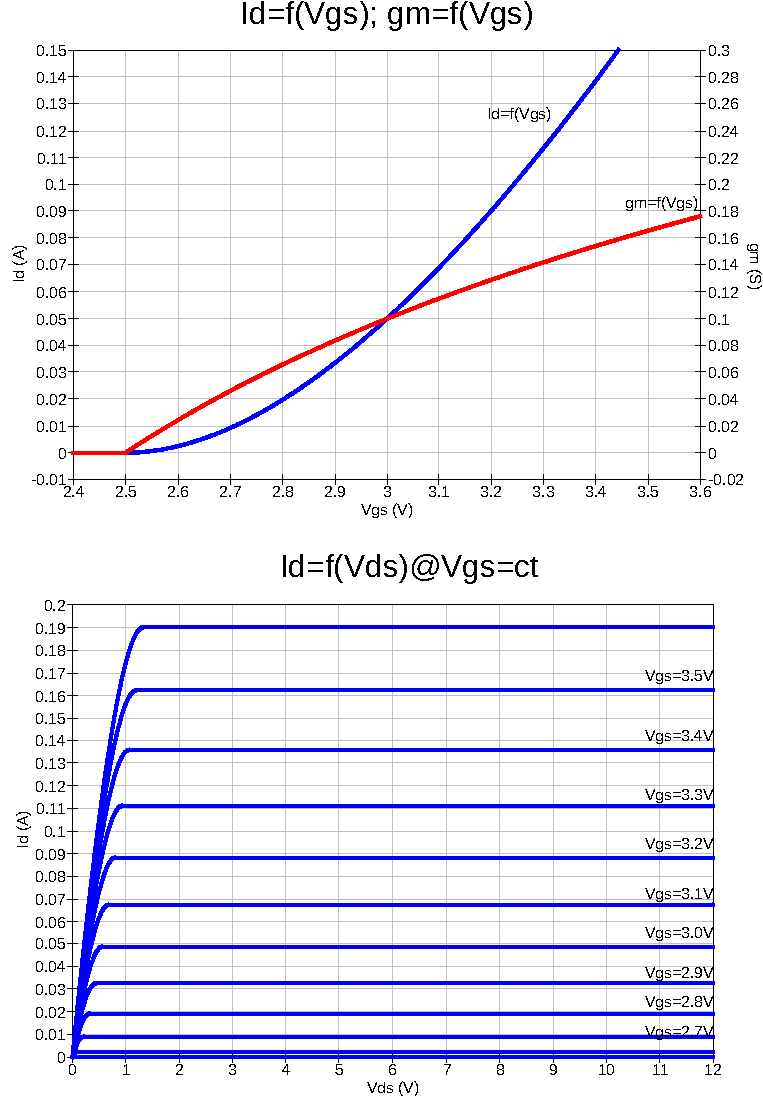
\includegraphics[width=17cm]{courbes_mos-crop.pdf}
%\end{center}

%QUESTION 1.
\Question
{
%question
%\textbf{
Sur base des courbes fournies, dimensionner la tension de polarisation $V_{dc}$ afin que l'étage amplificateur de tension ait un gain à vide $A_v=28.3dB$. 

%\\
%}
}
{%R
%-\\
\begin{enumerate}

	
	\item \fbox{$G=28.3dB$}\\
	
	Donc le gain en tension $A_v=\frac{V_{out}}{V_{in}}=\pm 10^{G/20}\approx \pm26$\\
	
	Or, on connaît le gain de cet étage à vide lorsqu'il est polarisé correctement :
	$V_{out}=-g_m R_D V_{in}$ 	
	
	d'où:	$A_v=-g_m R_D$
	
	Et on obtient donc la transconductance:
	$g_m=-\frac{A_v}{R_D}=\frac{-(-26)}{200\Omega}=0.13 S$
	
	\item \fbox{Courbe de transfert du transistor}\\
	
	On impose donc $g_m=0.13S$.\\
	Via la caractéristique de transfert $I_D=f(V_{GS})$ (et donc $g_m=f(V_{GS})$), on trouve $V_{GS}$.\\
%	\begin{center}
%		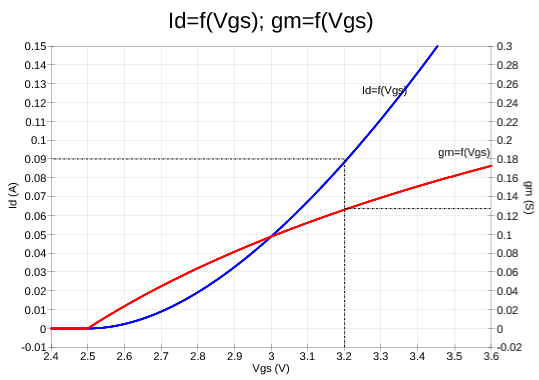
\includegraphics[width=10cm]{caract_mos_cor1.png}
%	\end{center}
	~\\
Selon la caractéristique, on a:\\
	$V_{GS}\cong 2.84V$\\
		
La tension de polarisation à la grille est:\\
	$V_{GS}=V_{DC}$ (pas de courant continu dans la résistance)\\
	
%De plus,\\
%	$V_{GSQ}=V_{GQ}-V_S=V_{GQ}+V_{CC}=V_{R2}$
%	
%Le diviseur résistif nous donne:\\
%	$V_{GSQ}=V_{R2}=\frac{R_2}{R_1+R_2}\left(V_{pol}-\left(-V_{CC}\right)\right)$\\
%	
%Donc:\\
%	$V_{pol}=\frac{R_1+R_2}{R_2}V_{GSQ}-V_{CC}=\frac{2R_2+R_2}{R_2}V_{GSQ}-V_{CC}$\\
	$\Rightarrow$ \fbox{$V_{DC}=2.84V$}
	
\end{enumerate}
}

%\Questiontsuite{Question 2.1. suite}{10cm}{8}
%{}
%{
%
%}

%\Questiontsuite{Question 2.1. suite}{8cm}{}
%{}
%{
%~\\
%Selon la caractéristique, on a :\\
%	$V_{GSQ}\cong 3.2V$\\
%	
%	Le diviseur résistif nous donne le potentiel de polarisation à la grille:\\
%	$V_{GQ}=\frac{R_2}{R_1+R_2}V_{pol}=\frac{R_2}{2R_2+R_2}V_{pol}=\frac{1}{3}V_{pol}$\\
%	
%	Avec:\\
%	$V_{GSQ}=V_{GQ}-V_S=V_{GQ}+V_{CC} \Leftrightarrow V_{GQ}=V_{GSQ}-V_{CC}=3,2-12=-8,8V$
%	
%	$\Rightarrow$ \fbox{$V_{pol}=3V_{GQ}=3*(-8,8)=-26,4V$}\\
%}

%QUESTION 2.
\Question
{%question
%\textbf{
Calculer la puissance dissipée par le transistor, due à la polarisation.

%}
}
{
~\\
\underline{\textbf{METHODE 1:}}\\

$V_{DS}=E-R_D\cdot I_{D}$\\
 
$P_{T}=V_{DS}\cdot I_{D}=\left(E-R_D\cdot I_{D}\right)I_{D}=E\cdot I_{D}-R_D\cdot I_{D}^2$\\
	
On connait la tension $V_{GS}=2.84V$. La caractéristique de transfert du transistor nous donne $I_{D}=25mA$ (voir page précédente).\\

$\Rightarrow$ \fbox{$P_{T}=E\cdot I_{D}-R_D\cdot I_{D}^2=175mW$}\\

\underline{\textbf{METHODE 2:}}\\

La réponse à la question précédente nous donne $V_{DS}=7V$.\\
$\Rightarrow$ \fbox{$P_{T}=V_{DS}\cdot I_{D}=7\times 0.025=175mW$}

}




%QUESTION 3.
\Question
{%question
%\textbf{
Vérifiez que le transistor reste bien dans sa zone de pincement si on impose à l'entrée de l'étage amplificateur une tension dont l'amplitude est bornée entre $-0.1V$ et $0.1V$.

}
{
~\\
Exprimons cette tension d'entrée comme suit :
$$v_{in}(t)=V_{in}\cdot fct(t)=\pm 0.1\cdot fct(t)$$

La tension de sortie sera donc comprise entre $-2.6V$ et $2.6V$ :
$$v_{out}(t)=V_{out}\cdot fct(t)=A_v\cdot v_{in}(t)= \pm 2.6\cdot fct(t)$$


On a donc une tension grille-source :
$$V_{GS}=V_{GS} + v_{gs}=V_{DC} + v_{in}(t)=2.84\pm 0.1\cdot fct(t)$$

Et une tension drain-source de polarisation :
$$V_{DS}=E-R_D\cdot I_{D}=7V$$

Ce qui nous donne le point de fonctionnement de la caractéristique de sortie du transistor $(I_{D};V_{DS})=(25mA;7V)$

De plus, l'équation suivante $V_{DS}=E-R_D\cdot I_{D}$ nous permet de trouver la droite de charge  passant par le point de fonctionnement:\\
$$I_D=-\frac{1}{R_D}V_{DS}+\frac{E}{R_D}=-0.005V_{DS}+60mA$$

En superposant cette droite de charge à la caractéristique de sortie, on voit que le dimensionnement convient puisqu'en zone de pincement, on dispose d'une excursion allant de $0.5V$ à $12V$ alors que le signal de sortie est compris entre $V_{DS}-2.6V$ et $V_{DS}+2.6V$.
\begin{center}
	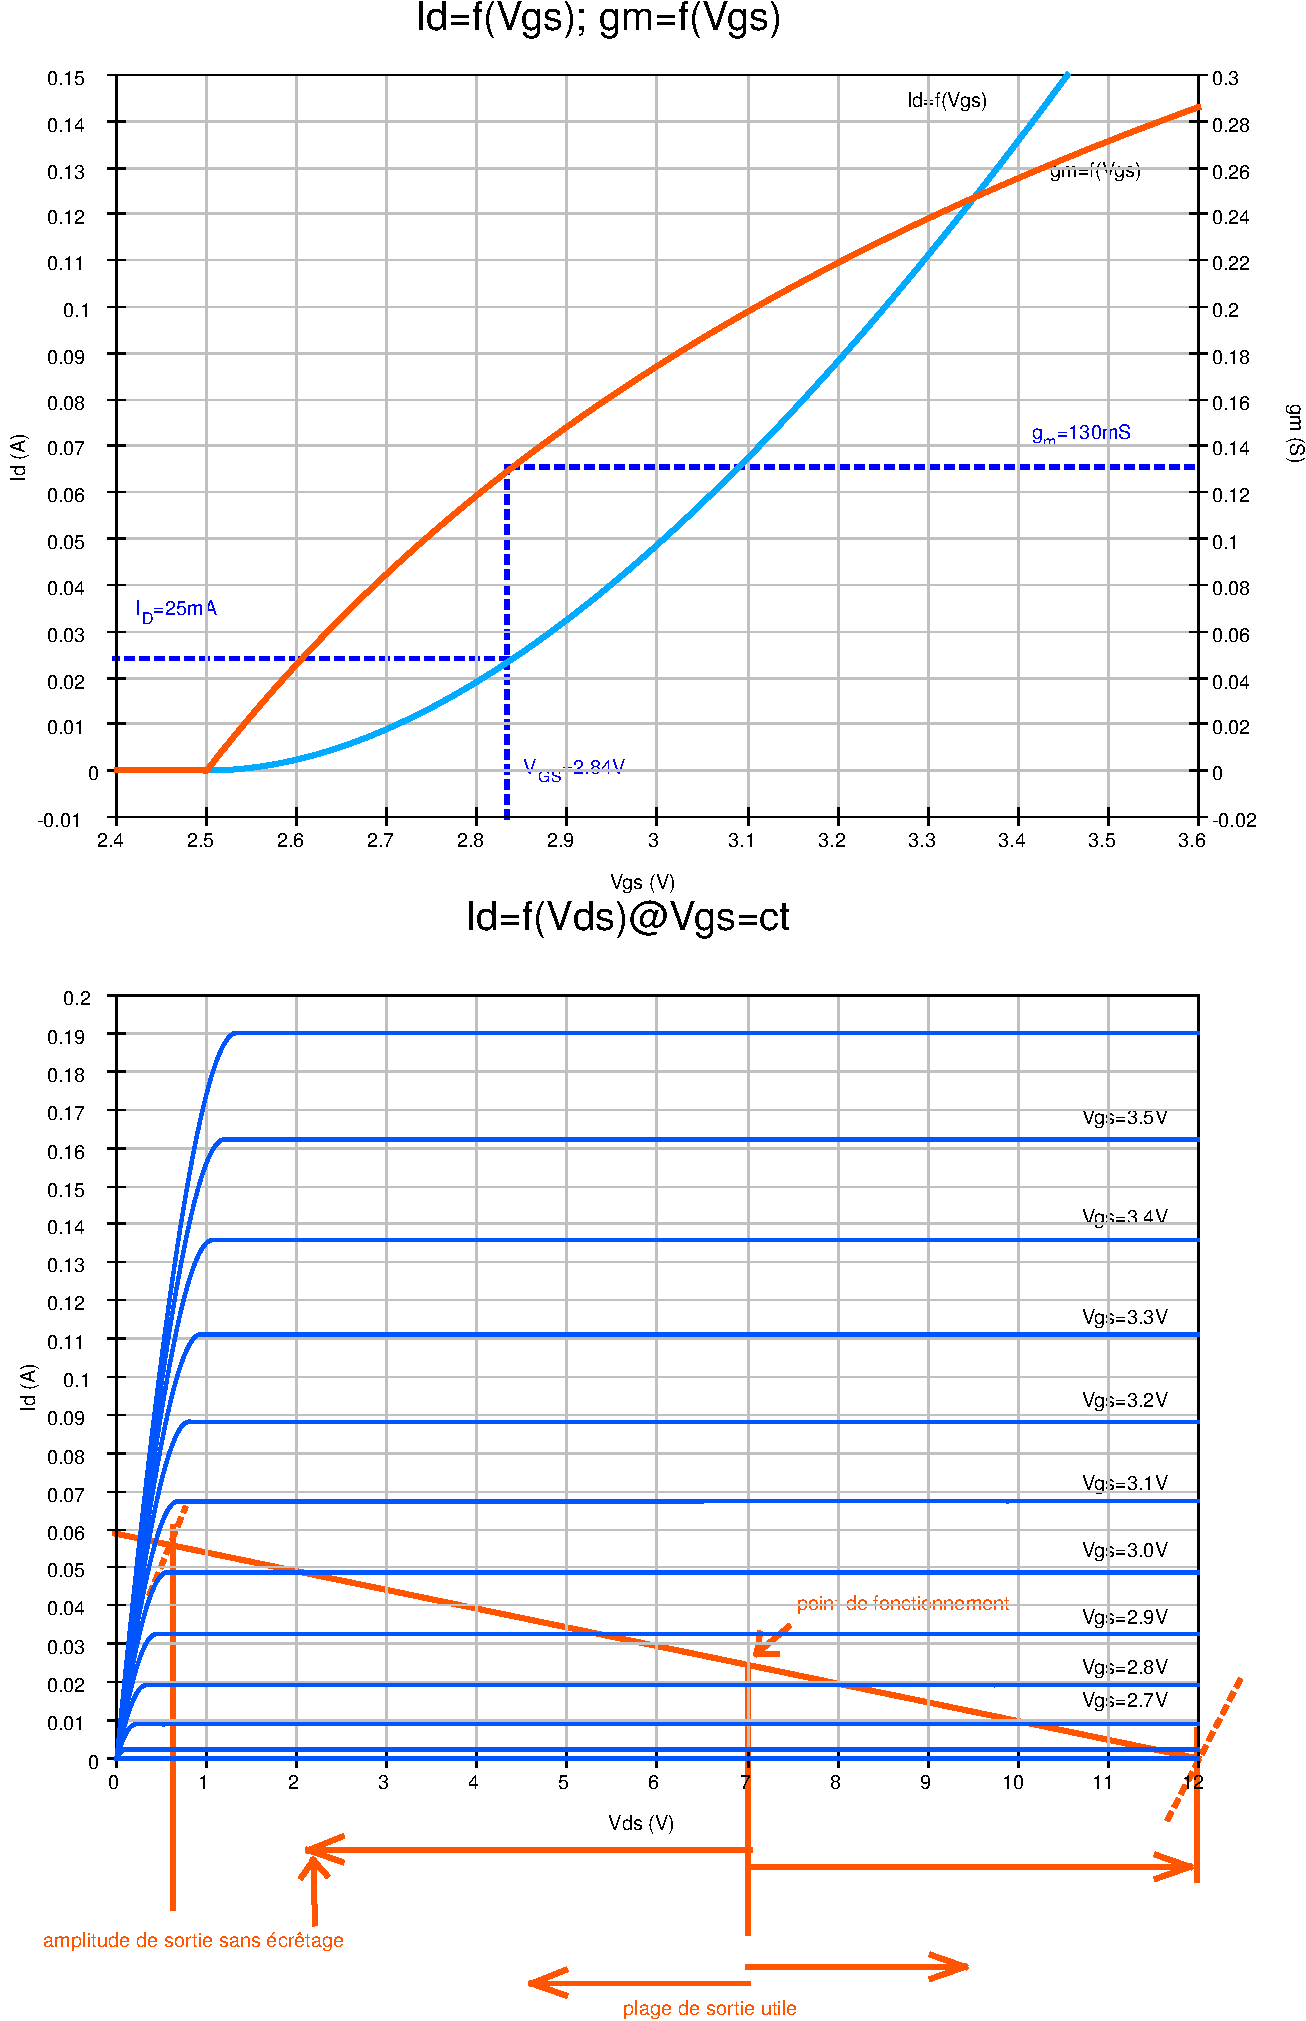
\includegraphics[width=10cm]{mos_exam_corr-crop.pdf}
%	\vspace{-5cm}
\end{center}
}
%\vspace*{-1cm}
%\newpage
\begin{center}
%\vspace*{-1cm}
%\hspace*{-0.8cm}
\ifgv{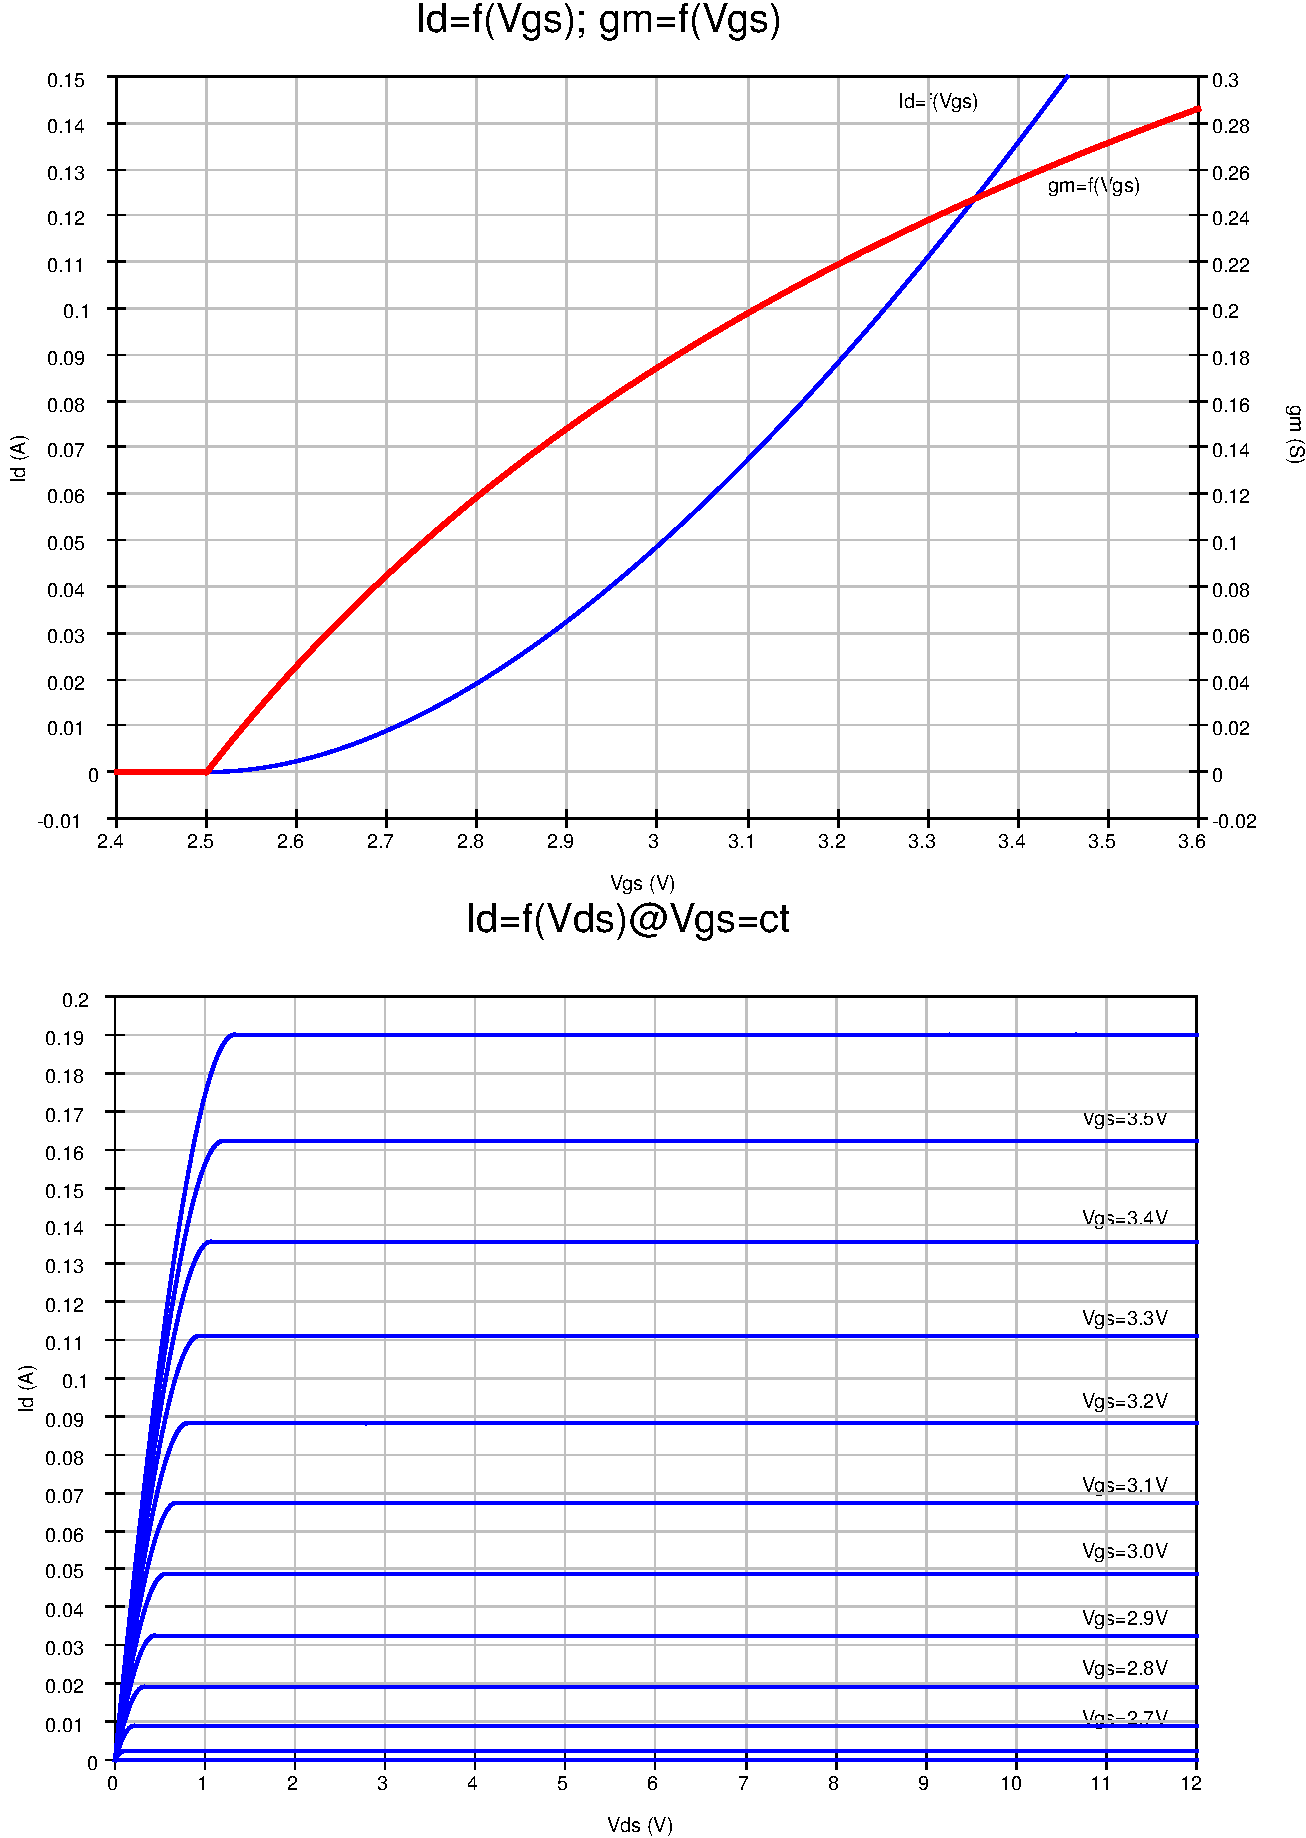
\includegraphics[width=16cm]{courbes_mos_2k16-crop.pdf}}
%\vspace*{-5cm}
\end{center}
%\newpage
%\vspace*{-10cm}
\appendix
\vspace*{-3cm}
\section{Caractéristiques}
%\subsection{BS170}
%\vspace*{-0.5cm}
\subsection{Caractéristiques du transistor NMOS BS170}
%\vspace{1cm}
\label{anx:mos_doc}
\begin{center}
\ifthenelse{\boolean{corrige}}
{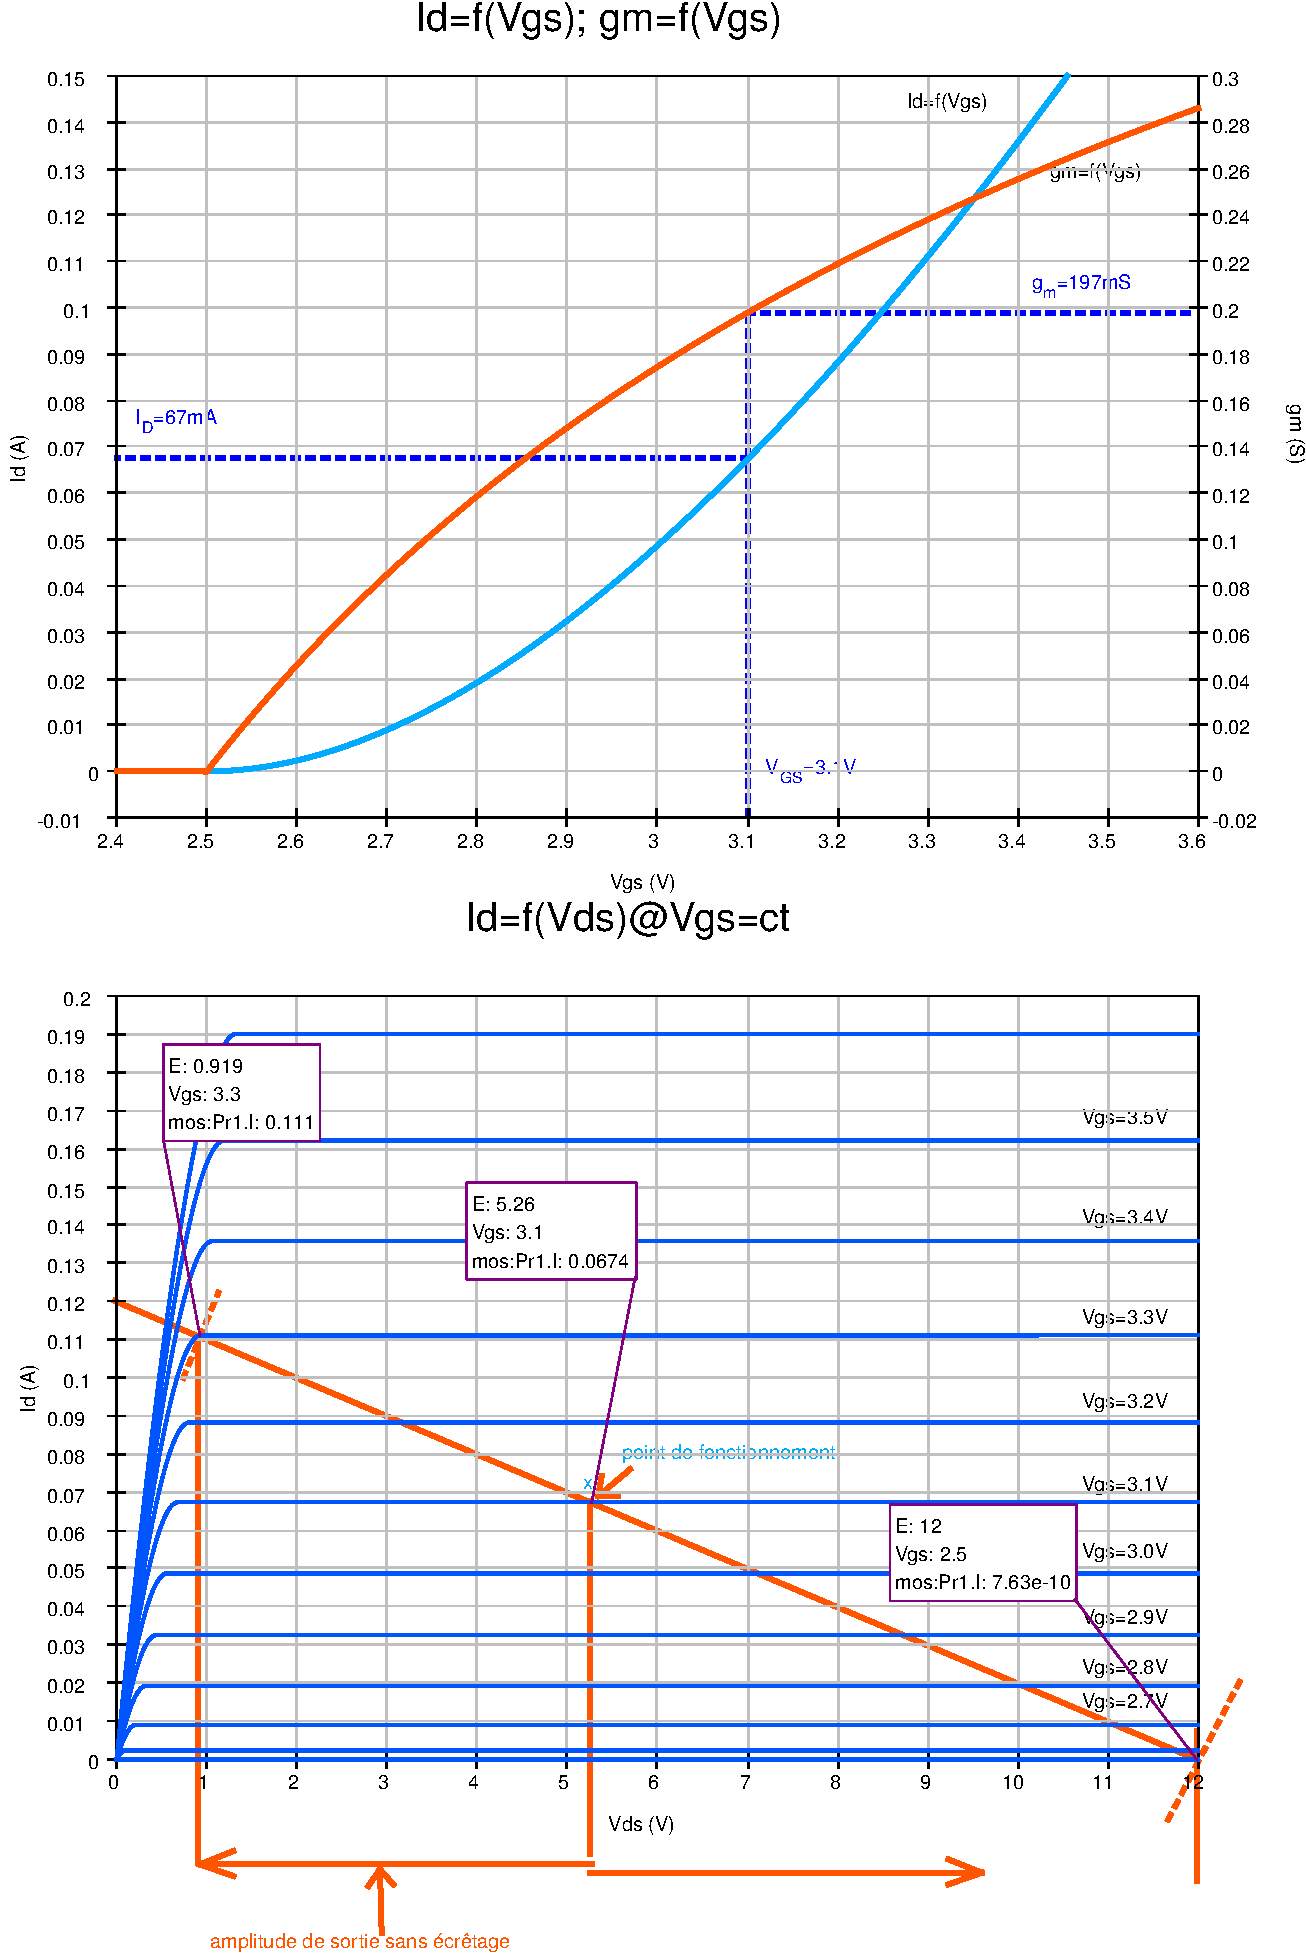
\includegraphics[width=15cm]{carac_mos_2k16_corr-crop.pdf}\vspace*{-5cm}}%then
{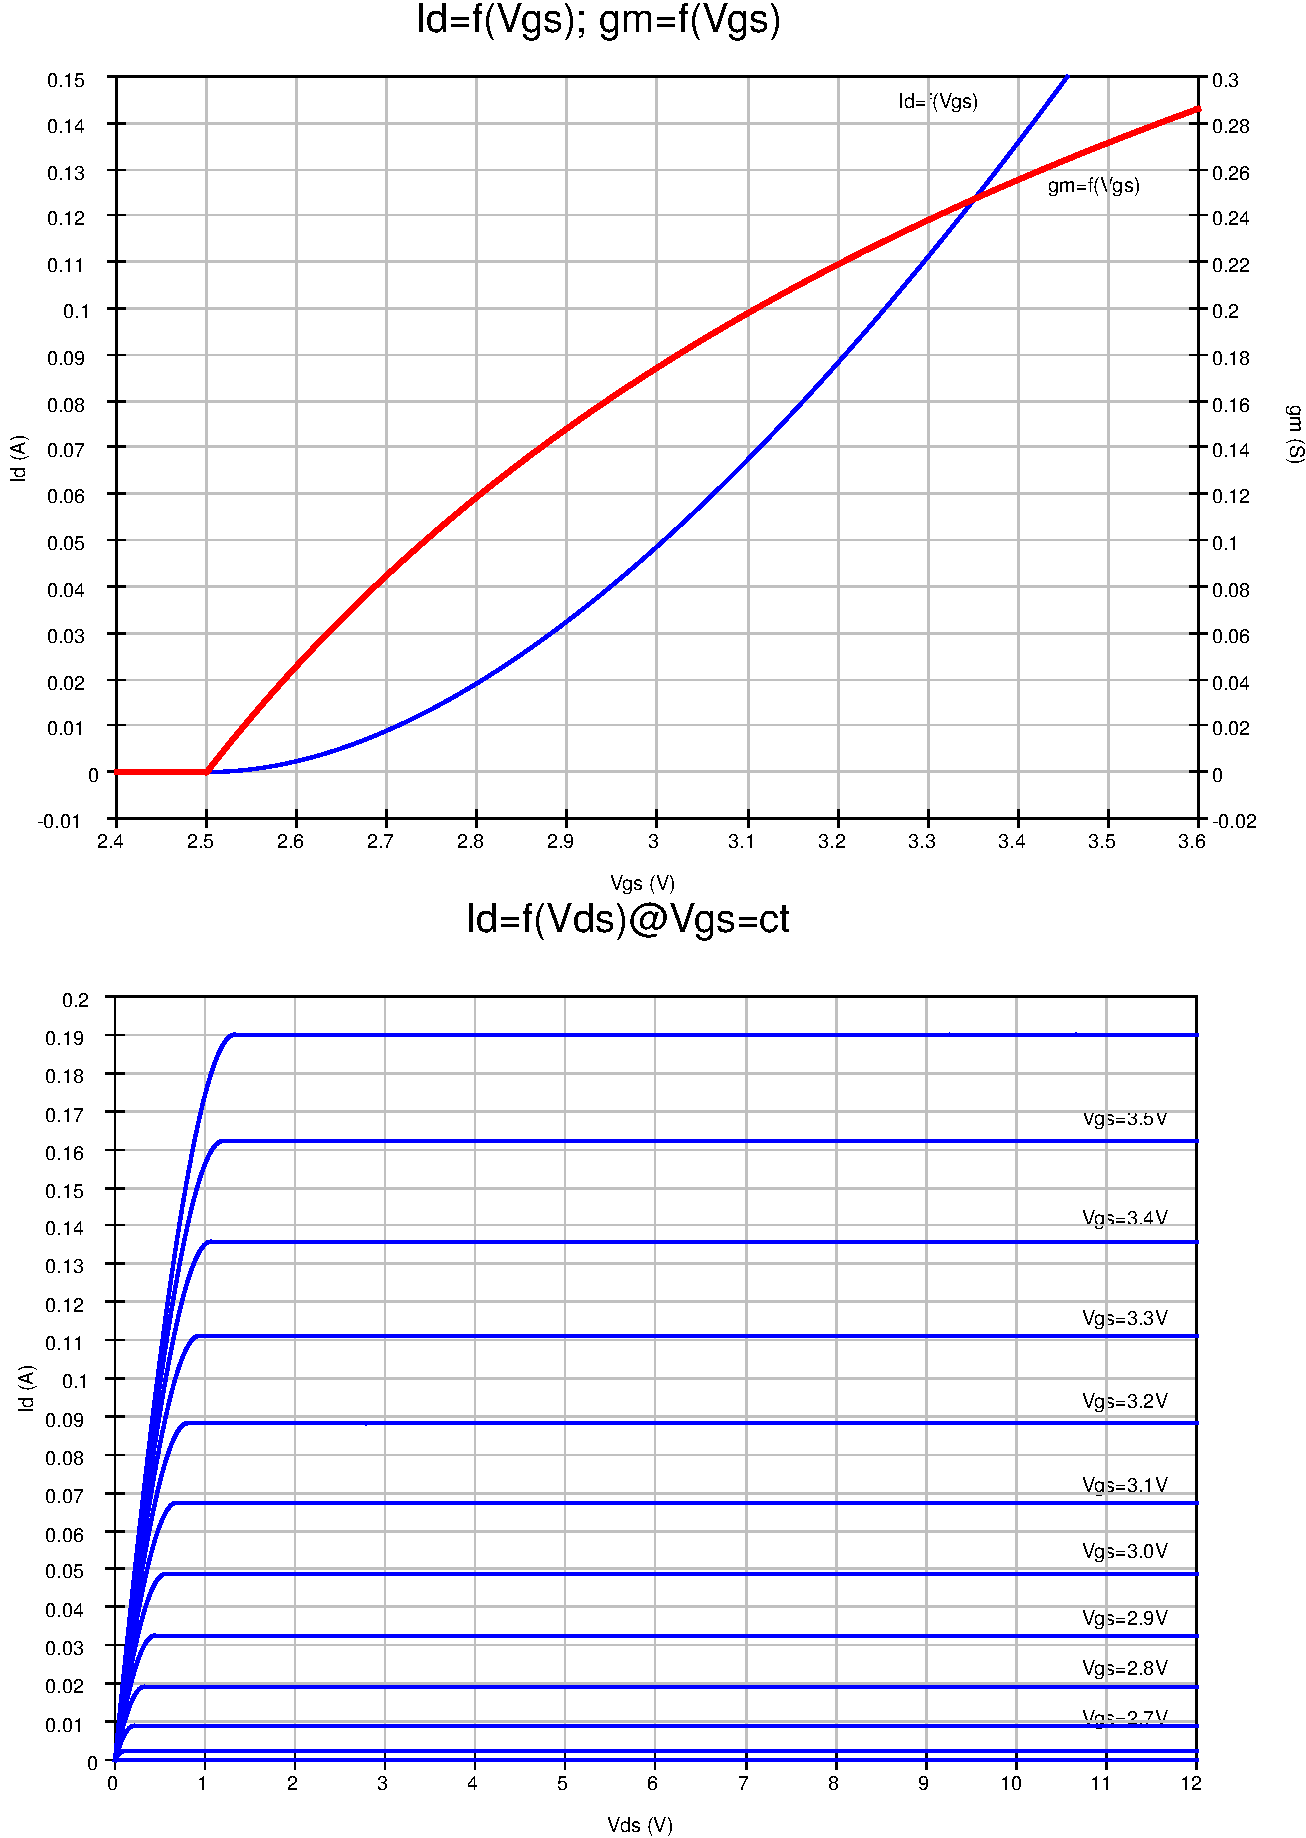
\includegraphics[width=16cm]{courbes_mos_2k16-crop.pdf}\vspace*{-5cm}}%else
% les courbes ici sont ont été corrigée et sont cohérentes.
\end{center}
%\vspace*{-3cm}
%\addcontentslinenono{toc}{section}{\href{http://pdf.datasheetcatalog.com/datasheets/70/123316_DS.pdf)}{\numberline{B}Documentation du transistor NMOS (lien cliquable)}}
%{\href{http://pdf.datasheetcatalog.com/datasheets/70/123316_DS.pdf}{\attachfile[icon=Graph, color=0 0.75 1,description =Documentation du transistor NMOS BS 170 ]{./Documentation_BS170.pdf}}}
%
%TODO : ajouter liens vers doc
%\vspace*{-2cm}
%\newpage
\subsection{BSL802SN}

%\begin{center}
\begin{center}
\ifthenelse{\boolean{corrige}}
{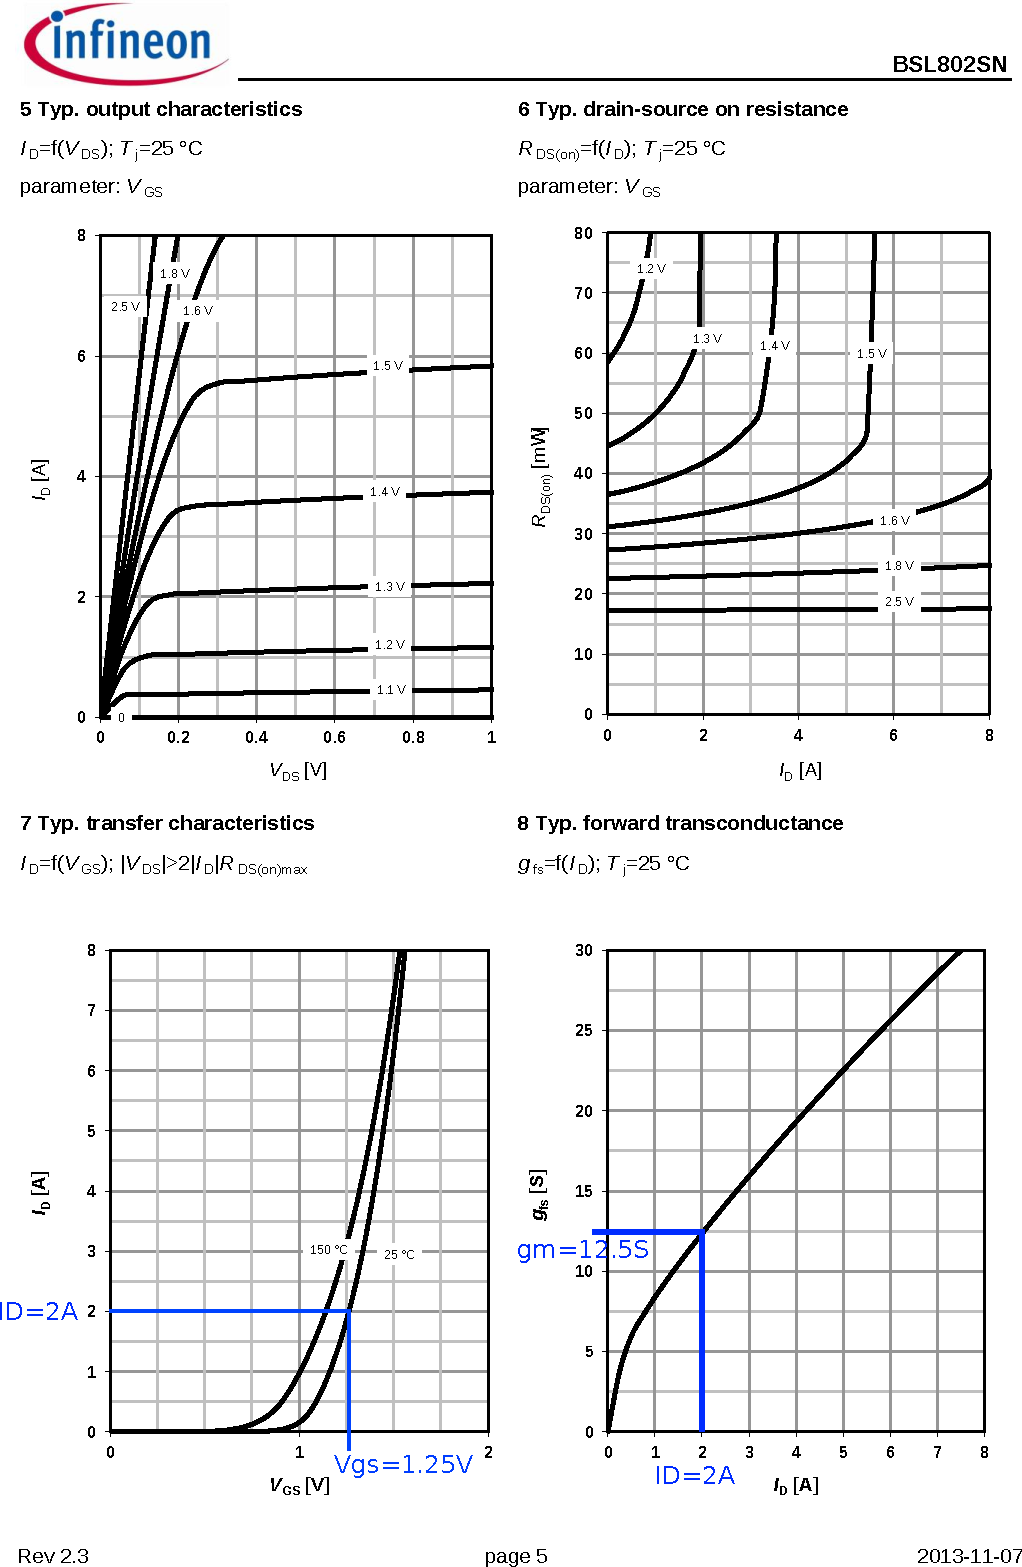
\includegraphics[width=15cm]{Infineon-BSL802SN-DS-v01_00-en_corr.pdf}}
{\vspace{-1cm}
\hspace{-1.5cm}\includegraphics[width=17cm,page=5]{Infineon-BSL802SN-DS-v01_00-en.pdf}}
\end{center}
%\end{center}
\vspace{-4cm}
% TODO : fancy header
\end{document}
